\documentclass{beamer}
\usetheme{CambridgeUS} %CambridgeUS
\usecolortheme{dolphin} %dolphin
%themes to test
%Theme to: AnnArbor Antibes Bergen Berkeley Berlin Boadilla boxes CambridgeUS Copenhagen Darmstadt default Dresden Frankfurt Goettingen Hannover Ilmenau JuanLesPins Luebeck Madrid Malmoe Marburg Montpellier PaloAlto Pittsburgh Rochester Singapore Szeged Warsaw
%Color to: albatross beaver beetle crane default dolphin dove fly lily orchid rose seagull seahorse sidebartab structure whale wolverine
%Font to: default professionalfonts serif structurebold structureitalicserif structuresmallcapsserif

\usepackage{graphicx} %allows picture file insertion into document
\usepackage{ulem} %allows strikethough (\sout)
\usepackage{amsmath}
\usepackage{comment}
\usepackage{multicol}

%sets numbered citation and uses bib.bib as bibliography file
\usepackage[natbib=true, style=numeric-comp, sorting=none]{biblatex}
\renewcommand*{\bibfont}{\tiny}
\addbibresource{../../../bibtex-sync/lectures-fluidResponsiveness.bib}
\newcommand{\pro}{\textcolor{blue}}
\newcommand{\con}{\textcolor{red}}

\setbeamerfont{footnote}{size=\tiny} %sets size of footnote citation to \tiny

\title{Assessing Fluid Responsiveness in the MICU}
\author{Eric W. Robbins}
\date{Last updated: \today}
\begin{document}
	\begin{frame}
		\maketitle
	\end{frame}
	\begin{frame}
		\frametitle{Table of Contents}
			\begin{multicols}{2}
				\tableofcontents
			\end{multicols}
	\end{frame}
	\section{Overview}
	\subsection{Scenario}
	\begin{frame}{A Common Scenario}
  		\begin{itemize}
  			\item Middle of the night in MICU.
  			\item Patient who has been in the ICU for several days with shock has increasing 	vasopressors requirements.
  			\item Senior (or fellow?) tells you to ``go ultrasound the IVC''.
  			\pause
  			\item Why?
  		\end{itemize}
	\end{frame}
	\subsection{The Goal}
	\begin{frame}{The Goal}
		\begin{itemize}
			\item Increase delivered oxygen ($DO_{2}$) and tissue perfusion / oxygenation
			\pause
				\begin{itemize}
					\item Abbreviations
						\begin{itemize}
							\item CO = cardiac output, HR = heart rate, SV = stroke volume, $DO_{2}$ = delivered oxygen, $CaO_{2}$ = oxygen content of the blood, Hgb = hemoglobin, SpO2 = pulse oximetry-derived oxygen saturation
						\end{itemize}
					\item \textbf{Formula / Definitions}
					\begin{itemize}
						\item $DO_{2}=(CO)\cdot (CaO_{2})$
						\pause
						\item $DO_{2}=(HR\cdot SV)\cdot(1.34\cdot[Hgb]\cdot SpO_{2})$
					\end{itemize}
				\end{itemize}
			\pause
			\item if $\uparrow$SV, we (may) $\uparrow$CO and (may) get $\uparrow$$DO_{2}$
			\item Notice all the ``mays'' in there.
		\end{itemize}
	\end{frame}
	\subsection{Physiology}
	\begin{frame}{Physiology}
		\begin{figure}
			\centering
			\includegraphics[height=0.8\textheight]{figures/frankStarling}
			\label{fig:frankstarling}
		\end{figure}
	\end{frame}
	\subsection{Some Thoughts}
		\begin{frame}{Some Thoughts}
			\begin{itemize}
				\item Fluid responsiveness $\neq$ patient should be get fluids!
					\begin{itemize}
						\item e.g., no shock
					\end{itemize}
				\pause
				\item However, if $\downarrow$ CO and requires correction:\\
				fluid responsiveness $\implies$ $\uparrow$SV (and usually $\uparrow$CO, unless HR falls) if fluids are given
			\end{itemize}
		\end{frame}
	\section{Assessing Shock}
		\subsection{Overview}
		\begin{frame}{Assessing Shock}{Overview}
			\begin{figure}
				\centering
				\includegraphics[height=0.8\textheight]{figures/shock-types}
				\label{fig:shock-types}
			\end{figure}
		\end{frame}
		\begin{frame}{Assessing Shock}{Distributive}
			\begin{figure}
				\centering
				\includegraphics[height=0.8\textheight]{figures/shock-distributive}
				\label{fig:shock-distributive}
			\end{figure}
		\end{frame}
	\section{Strategies}
			\begin{frame}{Strategies}{Overview}
				\begin{center}
					\begin{tabular}{l||l}
						\textbf{Static} & \textbf{Dynamic} \\	
						\hline
						\pause
						vital signs & passive leg raise\\
						\hline
						CVP / PCWP & end-expiratory occlusion test\\
						\hline
						``one off'' lactate / VBG & IVC ultrasound\\
						\hline
						pulse pressure variation & mini fluid challenge\\
					\end{tabular}
				\end{center}
			\end{frame}
			\begin{frame}{Strategies}{Overview}
				\begin{center}
					\begin{tabular}{l||l}
						\textbf{Static} & \textbf{Dynamic} \\	
						\hline
						\sout{vital signs} & \pro{passive leg raise}\\
						\hline
						\sout{CVP / PCWP} & \pro{end-expiratory occlusion test}\\
						\hline
						\sout{``one off'' lactate / VBG} & \pro{IVC ultrasound}\\
						\hline
						\pro{pulse pressure variation} & \pro{mini fluid challenge}\\
					\end{tabular}
				\end{center}
			\end{frame}
			\begin{frame}{Strategies}{Overview}
				\begin{center}
					\begin{tabular}{l||l}
						\textbf{Heart-Lung Interaction} & \textbf{Independent} \\	
						\hline
						\pro{pulse pressure variation} & \pro{passive leg raise}\\
						\hline
						\pro{end-expiratory occlusion test} & \pro{mini fluid challenge}\\
						\hline
						\pro{IVC ultrasound} & \\
					\end{tabular}
				\end{center}
			\end{frame}
\section{Monitoring Cardiac Output}
	\begin{frame}{Monitoring Cardiac Output}{Who do we know if we've helped?}
		\begin{itemize}
			\item \textbf{All} of these methods need a way to monitor cardiac output
			\item Most of these methods used \textit{non-invasive cardiac output monitoring (NICOM)} in studies
			\item We don't have NICOM systems at Brown
		\end{itemize}
	\end{frame}
	\begin{frame}{Monitoring Cardiac Output}{Overview}
		\begin{figure}
			\centering
			\includegraphics[height=0.8\textheight]{figures/nicom-overview}
			\label{fig:nicom-overview}
		\end{figure}
	\end{frame}
	\begin{frame}{Monitoring Cardiac Output}{Invasive Monitoring}
		\begin{figure}
			\centering
			\includegraphics[height=0.8\textheight]{figures/icom-sgc}
			\label{fig:icom-sgc}
		\end{figure}
	\end{frame}
	\begin{frame}{Monitoring Cardiac Output}{Less Invasive Monitoring}
		\begin{figure}
			\centering
			\includegraphics[height=0.8\textheight]{figures/icom-arterial-wave-analysis}
			\label{fig:icom-arterial-wave-analysis}
		\end{figure}
	\end{frame}
	\begin{frame}{Monitoring Cardiac Output}{Less Invasive Monitoring}
		\begin{figure}
			\centering
			\includegraphics[height=0.8\textheight]{figures/nicom-picco}
			\label{fig:nicom-picco}
		\end{figure}
	\end{frame}
	\begin{frame}{Monitoring Cardiac Output}{NICOM}
		\begin{figure}
			\centering
			\includegraphics[width=1.0\textwidth]{figures/nicom-ev1000}
			\label{fig:nicom-evo1000}
		\end{figure}
	\end{frame}
	\begin{frame}{Monitoring Cardiac Output}{NICOM}
		\begin{figure}
			\centering
			\includegraphics[width=1.0\textwidth]{figures/nicom-flotrac}
			\label{fig:nicom-flotrac}
		\end{figure}
	\end{frame}
	\begin{frame}{Monitoring Cardiac Output}{NICOM}
		\begin{figure}
			\centering
			\includegraphics[width=0.8\textwidth]{figures/nicom-lidcorapid}
			\label{fig:nicom-lidocopaid}
		\end{figure}
	\end{frame}
	\begin{frame}{Monitoring Cardiac Output}{NICOM}
		\begin{figure}
			\centering
			\includegraphics[height=0.8\textheight]{figures/tte-cardiacoutput}
			\label{fig:tte-cardiacoutput}
		\end{figure}
	\end{frame}
	\section{Assessment Methods}
		\subsection{Pulse Pressure Variation}
			\begin{frame}
				\begin{figure}
					\centering
					\includegraphics[height=0.90\textheight]{figures/ppv}
					\tiny Source: \cite{Teboul2019}
					\label{fig:ppv}
				\end{figure}
			\end{frame}
			\begin{frame}{Pros / Cons}{Pulse Pressure Variation}
				\begin{center}
					\begin{tabular}{l||l}
						\textbf{Pros} & \textbf{Cons} \\	
						\hline
						\pro{validated in intubated patients} & \con{not validated in non-intubated patients} \\
						\hline
						& \con{doesn't work in arrhythmias}\\
						\hline
						 & \con{not valid in tamponade}\\
					\end{tabular}
				\end{center} 
			\end{frame}
			\begin{frame}{Method}{Pulse Pressure Variation}
				\begin{itemize}
					\item $PPV=\cfrac{PP_{max}-PP_{min}}{\frac{PP_{max}-PP_{min}}{2}}=\cfrac{\Delta PP}{PP_{mean}}$
					\item Area under the curve $PPV=0.82$ \cite{AlvaradoSanchez2021}
				\end{itemize}
				\begin{figure}
					\centering
					\includegraphics[width=0.9\linewidth]{figures/responsivenessMethodsCompared-1}
					\label{fig:responsivenessmethodscompared-1}
				\end{figure}
			\end{frame}
		\subsection{Passive Leg Raise}
			\begin{frame}
				\begin{figure}
					\centering
					\includegraphics[width=0.95\linewidth]{figures/plr}
					\label{fig:plr}
				\end{figure}
				\tiny Source: \cite{Marik2011}
			\end{frame}
			\begin{frame}{Pros / Cons}{Passive Leg Raise}
				\begin{center}
					\begin{tabular}{l||l}
						\textbf{Pros} & \textbf{Cons} \\	
						\hline
						\pro{valid in intubated patients} & \con{body habitus}\\
						\hline
						\pro{valid in non-intubated patients} & \con{no legs!}\\
						\hline
						\pro{valid in arrhythmias} & \con{neurological injury}\\
						\hline
						\pro{may be more reliable than PPV} \cite{Monnet2012} & \con{no-turn patients}\\
					\end{tabular}
				\end{center} 
				 A prior Brown faculty member studied this, showing favorable outcomes when using PLR to guide resuscitation in septic shock \cite{Douglas2020}
			\end{frame}
			\begin{frame}{The Evidence}{Passive Leg Raise}
				\begin{itemize}
					\item Multiple studies showing good prediction ($AUR=0.84$) \cite{Monnet2006,AlvaradoSanchez2021}
					\begin{figure}
						\centering
						\includegraphics[width=0.9\linewidth]{figures/responsivenessMethodsCompared-2}
						\label{fig:responsivenessmethodscompared-2}
					\end{figure}
				\end{itemize}
			\end{frame}
		\subsection{End-Expiratory Occlusion Test}
			\begin{frame}
				\begin{figure}
					\centering
					\includegraphics[width=0.95\textwidth]{figures/eeot}
					\label{fig:eeot}
				\end{figure}
				\tiny Source: \cite{Gavelli2019}
			\end{frame}
			\begin{frame}{Pros / Cons}{End-Expiratory Occlusion Test}
				\begin{center}
					\begin{tabular}{l||l}
						\textbf{Pros} & \textbf{Cons} \\	
						\hline
						\pro{valid in intubated patients} & \con{requires significant sedation}\\
						\hline
						\pro{valid in $\downarrow$TV ventilation} & \con{can't do it in non-intubated patients}\\
						\hline
						\pro{valid in arrhythmias} & \con{respiratory stability}\\
					\end{tabular}
				\end{center}
			\end{frame}
			\begin{frame}{The Evidence}{End-Expiratory Occlusion Test}
				\begin{itemize}
					\item One meta-analysis found Area under the curve of $EEOT=0.92$!\cite{AlvaradoSanchez2021}
					\begin{figure}
						\centering
						\includegraphics[width=0.9\linewidth]{figures/responsivenessMethodsCompared-3}
						\label{fig:responsivenessmethodscompared-3}
					\end{figure}
					\item Multiple other studies have assessed it \cite{Gavelli2019}
				\end{itemize}
			\end{frame}
			\begin{frame}{Method}{Mini-Fluid Challenge}
				\begin{itemize}
					\item Rapidly infusion 100 cc of IV fluid
					\item Monitor stroke volume in real time
				\end{itemize}
				\begin{figure}
					\centering
					\includegraphics[height=0.7\textheight]{figures/lr}
					\caption{}
					\label{fig:lr}
				\end{figure}
				%\cite{Messina2019}
			\end{frame}
			\begin{frame}{Pros / Cons}{Mini-Fluid Challenge}
				\begin{center}
					\begin{tabular}{l||l}
						\textbf{Pros} & \textbf{Cons} \\	
						\hline
						\pro{less fluid overload} & \con{Requires precise cardiac output monitoring} \\
						\hline
						\pro{Good evidence it's predictive} & \con{Still requires giving fluid}
					\end{tabular}
				\end{center}
			\end{frame}
			\begin{frame}{The Evidence}{End-Expiratory Occlusion Test}
					\begin{figure}
						\centering
						\includegraphics[width=0.9\linewidth]{figures/responsivenessMethodsCompared-4}
						\label{fig:responsivenessmethodscompared-4}
					\end{figure}
			\end{frame}
		\subsection{IVC Ultrasound}
			\begin{frame}{IVC Ultrasound}{The Most Common Resident Assessment}
				\begin{itemize}
					\item This seems to me the one we use the most.
					\item What is it? How do we do it?
				\end{itemize}
			\pause
			\begin{figure}
				\centering
				\includegraphics[width=1.0\textwidth]{figures/ivc-external-view}
				\label{fig:fluidstrategy}
			\end{figure}
			\tiny{Images source} \cite{DeBacker2014}
			\end{frame}
			\begin{frame}{Why / how it works}
				\begin{itemize}
					\item if intra-abdominal pressure $\geq $ right atrial pressure, then IVC collapses
					\item Sniff test example
					\begin{itemize}
						\item acutely increases abdominal pressure
					\end{itemize}
				\end{itemize}
				\pause
				\begin{figure}
					\centering
					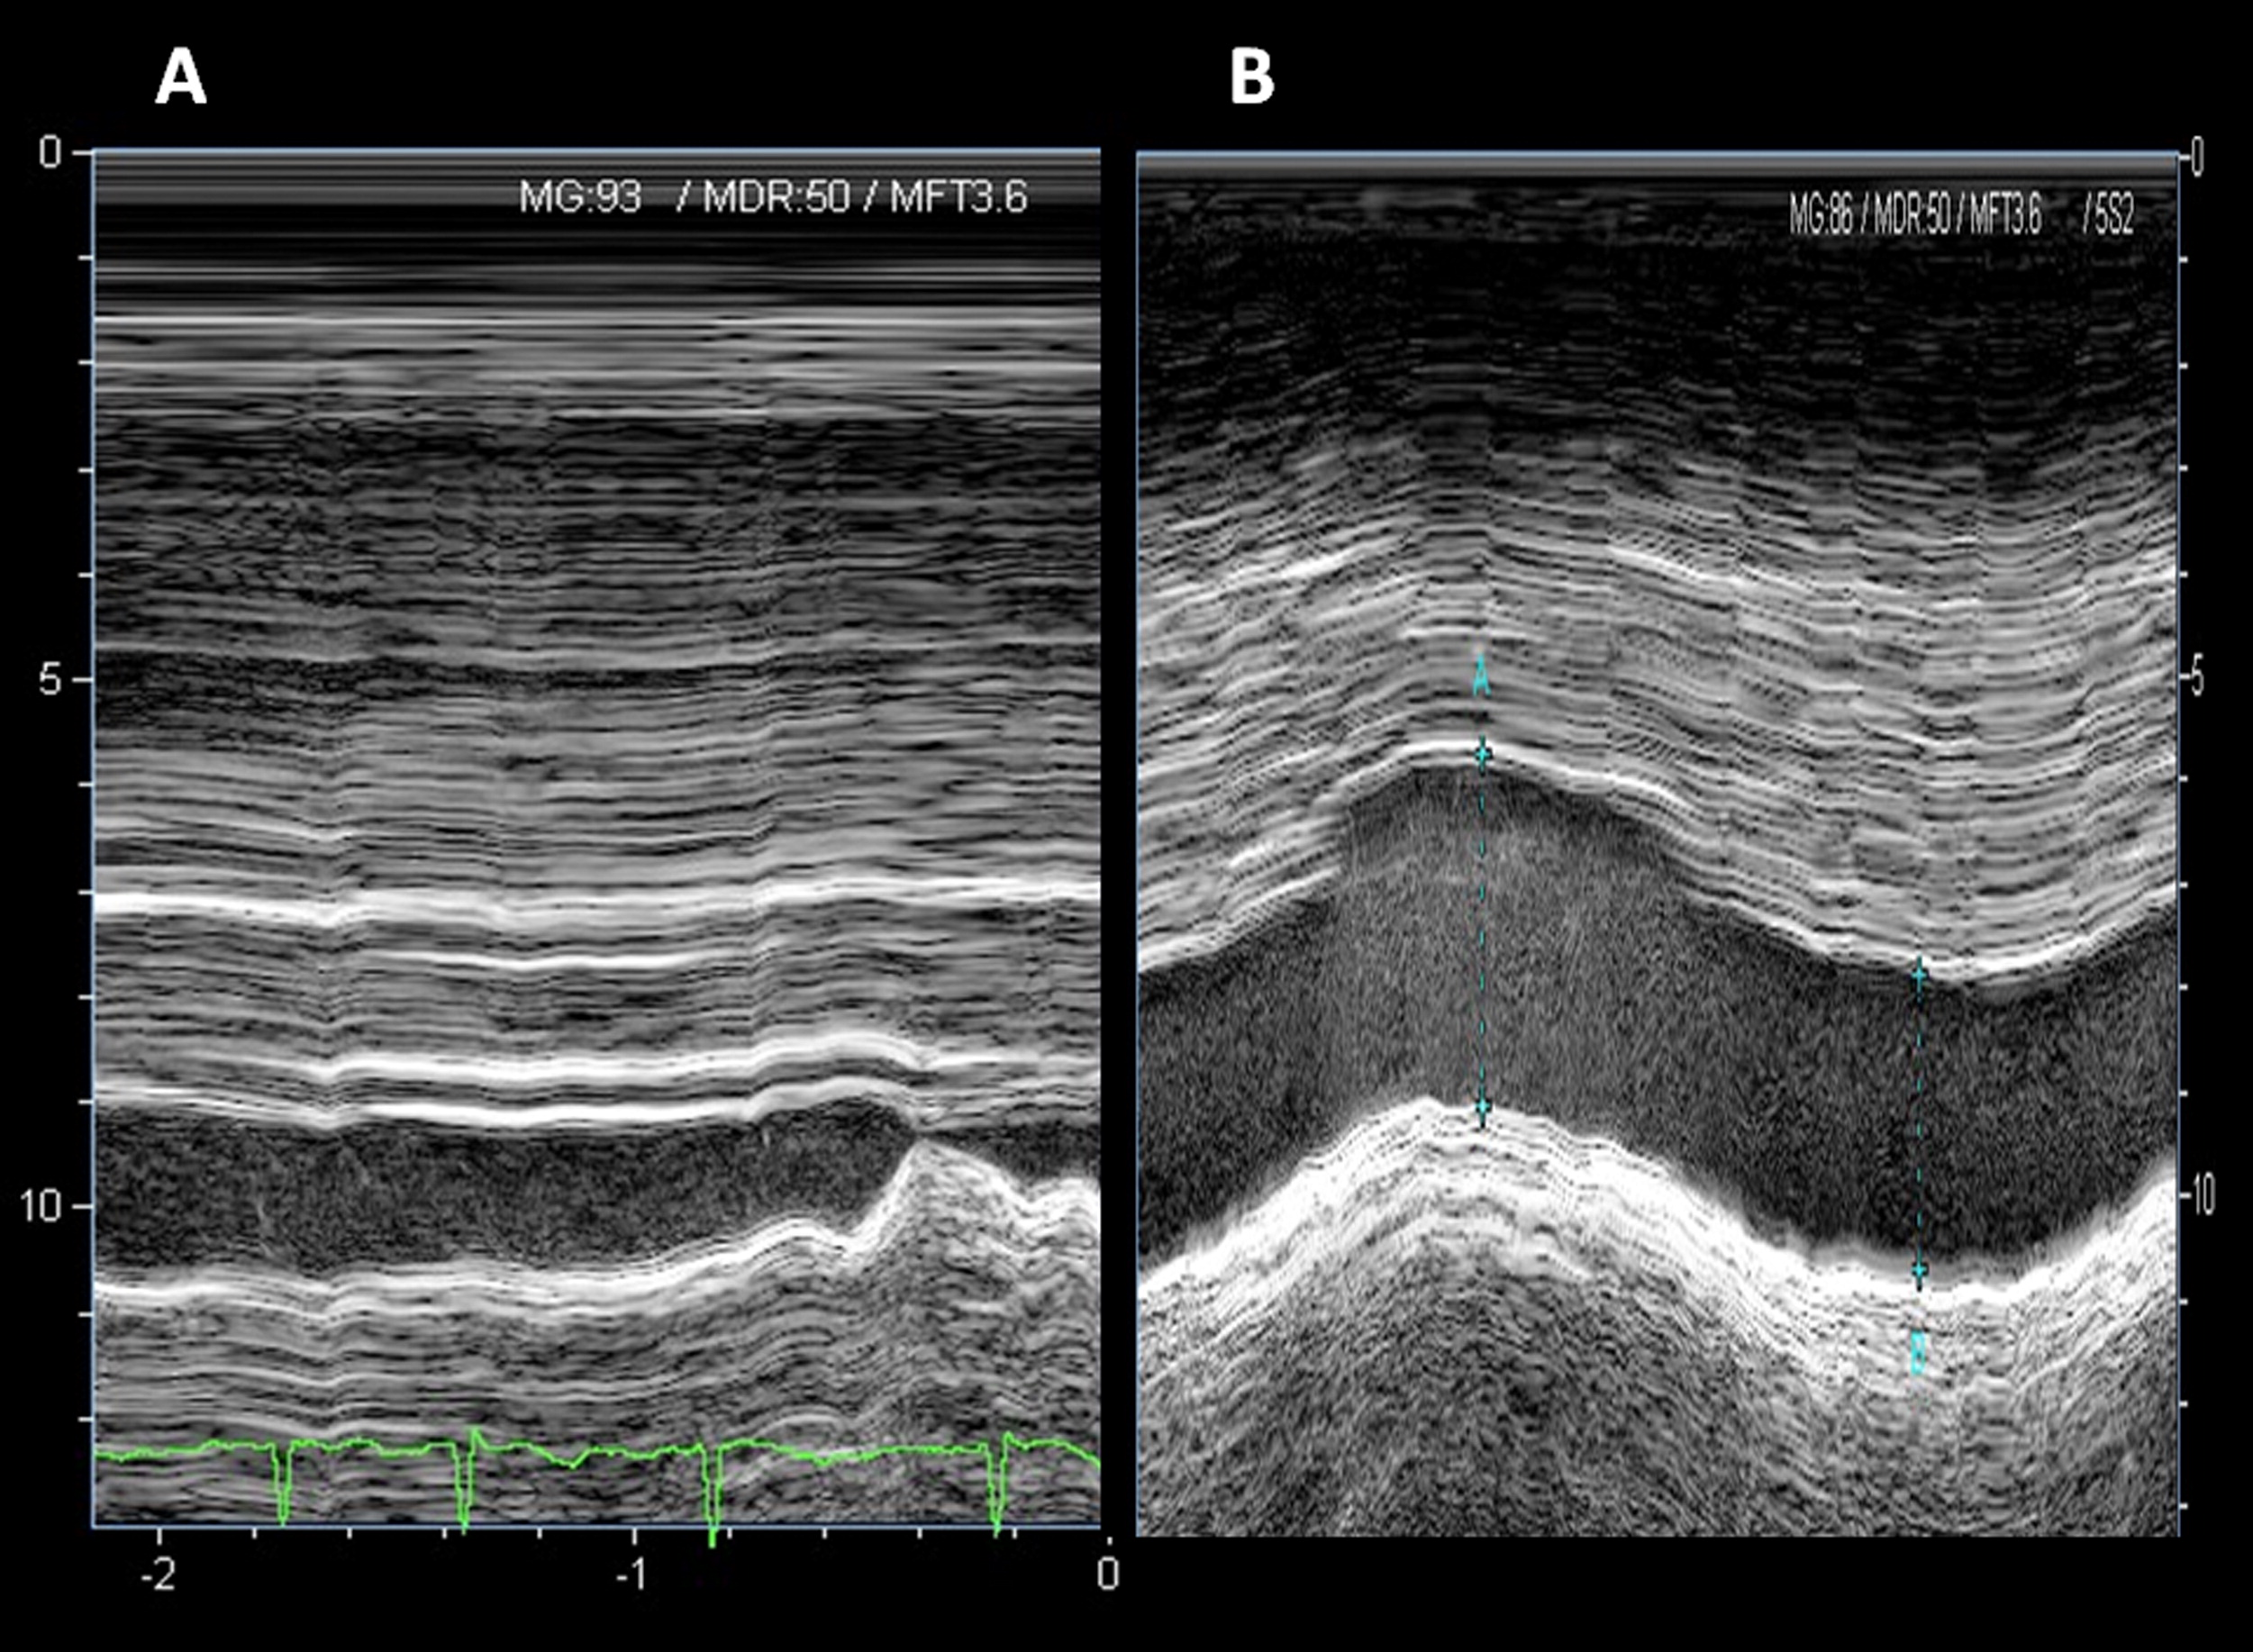
\includegraphics[height=0.6\textheight]{figures/ivc-collapse-noCollapse}
					\label{fig:fluidstrategy}
				\end{figure}
			\end{frame}
			\begin{frame}
				\begin{figure}
					\centering
					\includegraphics[width=0.95\textwidth]{figures/ivc-view-labeled}
					\label{fig:fluidstrategy}
				\end{figure}
			\end{frame}
			\begin{frame}
				\begin{figure}
					\centering
					\includegraphics[width=0.95\textwidth]{figures/ivc-respiratory-variation}
					\label{fig:fluidstrategy}
				\end{figure}
			\end{frame}
			\begin{frame}{Pros / Cons}{IVC Ultrasound}
				Lots of limitations (source:\cite{Via2016}):
				\pause
				\begin{center}
					\begin{tabular}{l||l}
						\textbf{Pros} & \textbf{Cons} \\	
						\hline
						\pro{valid in intubated patients} & \con{inconsistencies in non-intubated patients}\\
						\hline
						\pro{easy to administer} & \con{not valid in $\uparrow$ PEEP and/or $\downarrow$ TVs}\\
						\hline
						\pro{} & \con{can't use in several heart issues}\\
						\hline
						\pro{} & \con{can't use with increased abdominal pressure}\\
						\hline
						\pro{} & \con{IVCs don't uniformly collapse}\\
						\hline
						\pro{} & \con{inspiration can laterally displace IVC}
					\end{tabular}
				\end{center}
			\end{frame}
			\begin{frame}{Quality of Evidence}{IVC Ultrasound}
				\begin{itemize}
					\item PubMed has indexed 3 systematic reviews \cite{Long2017,Orso2020,Kim2021}
					\begin{itemize}
						\item Long2017: ``Respiratory variation in IVC diameter has \textbf{limited ability to predict fluid responsiveness}, particularly in spontaneously ventilating patients. A negative test cannot be used to rule out fluid responsiveness.''
						\item Orso2020: ``Ultrasound evaluation of the diameter of the IVC and its respiratory variations \textbf{does not} seem to be a reliable method to predict fluid responsiveness.''
						\item Kim2021: ``Our results suggest that the \textbf{diagnostic accuracy ... is acceptable}.'' 
						\begin{itemize}
							\item Sensitivity 0.75, specificity 0.83, positive likelihood ratio 4.37, negative likelihood ratio - 0.30, Area under the curve 0.86
						\end{itemize}
					\end{itemize}
					\item caveat: first two had \con{spontaneously breathing} patients
				\end{itemize}
			\end{frame}
			\begin{frame}{Quality of Evidence}{IVC Ultrasound}
				\begin{itemize}
					\item PubMed only has 2 RCTs looking at fluid responsiveness using ultrasound and IVC variation
						\begin{itemize}
							\item both in patients before and after getting spinal anethesia
							\item mixed results (\cite{Ceruti2018,Tawfik2019})
						\end{itemize}
				\end{itemize}
				\begin{figure}
					\centering
					\includegraphics[width=0.9\linewidth]{figures/responsivenessMethodsCompared-all}
					\label{fig:responsivenessmethodscompared-all}
				\end{figure}
			\end{frame}
	
	\section{Conclusions}
		\begin{frame}{Conclusions}
			\begin{itemize}
				\item Remember to evaluate type of shock
				\item \con{Fluid responsiveness $\neq$ patient should be get fluids!}
				\item Remember this limitations of each method
					\begin{itemize}
						\item \pro{Passive leg raise has fewest limitations}
						\item For intubated patients, EEOT and mini-fluid challenge are good
						\item IVC ultrasound isn't bad either
					\end{itemize}
				\item Don't forget to monitor cardiac output!
			\end{itemize}
		\end{frame}
\section{References}
	\begin{frame}{Post-Lecture Survey}
		\begin{figure}
			\centering
			\includegraphics[height=0.8\textheight]{figures/qr}
			\label{fig:qr}
		\end{figure}
	\end{frame}
	\begin{frame}[allowframebreaks]{References} %option allowframebreaks gives page break to allow all references to not be on a single page
		\printbibliography
	\end{frame}
\end{document}

%refs
%10.1007/s12471-013-0487-7 (Basic concepts of fluid responsiveness)
%10.1186/s13613-016-0216-7 (Prediction of fluid responsiveness: an update)
%10.1186/s13613-021-00817-5 (Predictors of fluid responsiveness in critically ill patients mechanically ventilated at low tidal volumes: systematic review and meta-analysis)